%%%%%%%%%%%%%%%%%%%%%%%%%%%%%%%%%%%%%%%%%%%%%%%%%
%%%
%%% Auteur : Stéphane Péchard - stephane.pechard@univ-nantes.fr
%%% Fichier : 6-methode.tex - sixième chapitre : Méthode des tubes
%%% Version : 0.1
%%% Date : 2007/07/30
%%%
%%%%%%%%%%%%%%%%%%%%%%%%%%%%%%%%%%%%%%%%%%%%%%%%%
\chapter{Méthodologie d'évaluation subjective de l'impact d'un système dégradant sur la qualité visuelle} \label{chap:methode}
% \opt{final}{\lettrine[lines=4]{D}{iffuser de la télévision haute définition}}\opt{nofinal}{Diffuser de la télévision haute définition} nécessite le transport d'une très grande quantité d'information. À la base, sans faire appel aux techniques de compression d'information, celle-ci est multipliée par cinq par rapport à la TVSD. C'est pourquoi la compression est indispensable à la mise à disposition d'un tel service. Le débit de la TVHD 1080i avant compression est d'environ 800 Mbps, rien que pour la vidéo. Parallèlement, les débits visés pour la diffusion de la TVHD sont de l'ordre de 10 Mbps. Il faut donc réduire de façon très importante la quantité d'information à transmettre d'un facteur d'au moins 80. En pratique, un facteur 100 est visé. La première génération de TVHD actuellement utilisée aux États-Unis ou au Japon utilise la norme de compression MPEG-2. Pour sa généralisation en Europe, il est prévu d'utiliser la norme \avc, aussi appelée MPEG-4/Advanced Video Coding. Plus récente et plus performante, celle-ci permet de diviser les débits MPEG-2 par deux à qualité visuelle équivalente. Évidemment, une telle compression des données affecte quelque peu le rendu visuel. En effet, les techniques de compression sans perte ne réduisent le débit que d'un facteur deux environ, taux de compression très insuffisant. Il faut se résoudre à utiliser, comme le fait MPEG-2, des techniques de compression avec pertes. Vu les taux de compression utilisés, les distorsions dues à la compression deviennent visibles. La qualité visuelle de l'image est donc affectée. La perte d'information est alors perçue par l'observateur sous la forme d'apparition de phénomènes dégradants spatiaux et temporels non réalistes.

% Mesurer ces dégradations permet d'en déterminer l'impact sur la qualité visuelle. Or, pour un débit donné, le but d'un système moderne de compression d'information est de minimiser les dégradations qu'il génère. Il semblerait donc logique de pouvoir calculer la quantité de dégradations en fonction du débit et utiliser cette relation pour déterminer la qualité perçue correspondant à un certain débit. Ce n'est malheureusement pas aussi élémentaire. En effet, la relation entre la qualité ressentie et le niveau des dégradations n'est pas simple du fait de la diversité des dégradations mais aussi et surtout car elle fait intervenir un élément très complexe : le jugement humain. Nous remarquons que les systèmes de codage n'optimisent pas leurs procédés selon l'impact que ceux-ci peuvent avoir sur le jugement humain mais plutôt selon des paramètres statistiques élémentaires basés sur des différences entre signaux numériques d'entrée et de sortie. Or, il est connu que les appréciations issues du jugement humain et ces paramètres statistiques élémentaires ne sont pas très corrélées.

\opt{final}{\lettrine[lines=4]{I}{l existe plusieurs approches pratiques possibles}}\opt{nofinal}{Il existe plusieurs approches pratiques possibles} pour mesurer de manière subjective les dégradations générées par un système dégradant. Celles que nous avons présentées dans le premier chapitre étaient globales, c'est-à-dire qu'elles considéraient la séquence dans son entier et que le système dégradant s'appliquaient entièrement sur la séquence. Nous proposons ici une approche plus fine. Il existe d'autres méthodes adoptant une approche fine~\cite{farias-phd,eusipco2006-wolff} mais elles utilisent une classification des dégradations présentes dans la séquence. Ce type de méthode suppose une mesure indépendante de chaque dégradation, ce qui n'est pas sans soulever quelques problèmes pratiques.

Dans ce chapitre, nous présentons une méthodologie permettant d'estimer l'impact de dégradations de codage sur la qualité perçue par l'observateur moyen. L'approche envisagée s'inspire des travaux de Farias~\cite{farias-phd}. Cependant, nous préférons ne pas considérer plusieurs types de dégradations qui seraient appliqués arbitrairement sur tout ou partie d'une séquence vidéo. Nous renversons cette approche en considérant un unique type de dégradation provenant du codage, au lieu d'une liste de dégradations qu'il est difficile de déterminer étant donné la diversité des conséquences visibles d'un processus de compression. Dans un second temps, nous exploiterons la méthodologie pour rechercher une éventuelle relation entre les pertes de qualité locales et la perte de qualité globale. %Cependant, nous considérons que cette dégradation s'applique de manière différente suivant l'activité spatio-temporelle locale du contenu. Nous passons donc d'un partitionnement des dégradations en type à un partitionnement du contenu en zones spatio-temporelles. Pour cela, nous proposons une méthode de classification spatio-temporelle d'un contenu vidéo. Chaque partie obtenue est ensuite dégradée et évaluée indépendemment. Dans notre contexte, nous restreignons notre étude aux dégradations introduites pas le système de codage \avc. Une fois que nous disposons des pertes de qualité de chaque type de contenu, nous essayons de savoir si il est possible de les relier avec la perte de qualité globale. Un tel résultat serait très intéressant dans l'optique d'un critère objectif de qualité. Dans un second temps, nous cherchons à créer un paramètre de contrôle de dégradation par type de contenu. Celui-ci permet alors de construire un modèle de perte de qualité basé sur une fonction de gêne.


\section{Vers une classification du contenu et non des dégradations}
Avant de décrire notre méthode de classification spatio-temporelle et de l'exploiter, nous commençons par détailler l'approche proposée par Farias, dont nous nous inspirons. Elle utilise sa méthode pour mesurer les dégradations présentes dans une vidéo codée par MPEG-2 et créer des critères objectifs de qualité. Nous expliciterons ensuite les défauts dans la réalisation de la méthode et les modifications que nous nous proposons d'y apporter afin de mieux répondre à la problématique.


\subsection{Approche de Farias}
Farias~\cite{farias-phd} propose de considérer une liste de dégradations et de tester leur influence sur la qualité perçue suivant la tâche demandée à l'observateur. La figure~\ref{fig:approcheFarias} présente une schématisation simplifiée de cette approche. Les dégradations considérées sont :
\begin{itemize}
\item l'effet de bloc, dû à l'apparition d'incohérences spatiales sur les bords des blocs d'image, unité de base utilisée par le codeur ;
\item le flou, dû à la perte de détails spatiaux ;
\item le bruit, motif non prévisible de faible intensité ;
\item l'effet \emph{ringing}, apparition d'oscillations irrégulières le long des contours.
\end{itemize}

Elles correspondent aux phénomènes majeurs liés à un système de codage MPEG-2. Chaque dégradation est synthétisée par des traitements de bas niveaux comme par exemple un filtre moyenneur pour générer le flou. L'étape suivante est d'appliquer ces traitements à des contenus originaux de manière individuelle ou combinée. L'auteur réalise ceci par zones spatiales de l'image. Une zone de dégradation est définie par la région spatio-temporelle de la séquence où la dégradation est appliquée. La localisation de ces zones est arbitraire, il peut s'agir par exemple de trois rectangles verticaux de même taille. Dans l'exemple de la figure~\ref{fig:approcheFarias}, seule la partie gauche est utilisée. Cette pratique est justifiée par le fait qu'elle évite aux observateurs de se rappeler où se situent les dégradations. Plusieurs tâches sont demandées aux observateurs lors des tests subjectifs. Huit campagnes de test différentes regroupent des actions de détection, de mesure de gêne, de description et de mesure d'intensité des dégradations insérées sur une ou des combinaisons de plusieurs dégradations synthétiques. L'ensemble de ces tâches permet de construire des fonctions de gêne en fonction de chaque dégradation ou de certaines combinaisons. Ces fonctions permettent de localiser la qualité perçue dans l'espace multi-dimensionnel des dégradations retenues. Cette caractérisation permet ensuite de concevoir des métriques de qualité liées à ces dégradations, dans un contexte de codage MPEG-2 pour la télévision standard. La métrique consiste à mesurer dans une séquence codée la contribution de chaque type de dégradation. Le cumul est ensuite obtenu par combinaison des contributions. La loi de combinaison est construite grâce aux résultats des tests subjectifs. De plus, l'utilisation de dégradations synthétiques permet de disposer des paramètres de chaque traitement. Il est donc aisé de les utiliser pour contrôler l'intensité des dégradations et donc obtenir leurs fonctions de gêne. Cette possibilité est un avantage indéniable de la méthode.

\begin{figure}[htbp]
	\centering
	\begin{tikzpicture}[text centered]% \begin{tikzpicture}[text centered]
	\draw[legende] (-3.25,2.5) rectangle (11.25,-4);
	\node at (4,2.1) {\strong{création de séquences dégradées par partie avec des dégradations synthétiques}};
	\node at (0,0) {\includegraphics[width=6cm]{img/chap3/aboveMarathonFlou}};
	\draw (-1,1.7) -- (-1,-1.7);
	\node at (-2,1.2) {flou};
	\node at (4,0) {\includegraphics[width=6cm]{img/chap3/aboveMarathonBloc}};
	\draw (3,1.7) -- (3,-1.7);
	\node at (2,1.2) {effet de bloc};
	\node at (8,0) {\includegraphics[width=6cm]{img/chap3/aboveMarathonBruit}};
	\draw (7,1.7) -- (7,-1.7);
	\node at (6,1.2) {bruit};
	\node at (2.5,-2) {\includegraphics[width=6cm]{img/chap3/aboveMarathonFlouBruit.png}};
	\draw (1.5,-0.3) -- (1.5,-3.7);
	\node at (0.5,-0.8) {bruit+flou};
	\node at (5.5,-2) {\includegraphics[width=6cm]{img/chap3/aboveMarathonBlocFlou.png}};
	\draw (4.5,-0.3) -- (4.5,-3.7);
	\node[text width=1.5cm] at (3.5,-0.8) {effet de bloc+flou};
	\node at (9,-2) {\dots};

	\node[action,text width=6cm] (node) at (0,-5.5) {tests de détection, description, mesure de gêne et d'intensité};
	\draw[fleche] (0,-4) -- (node);
	\draw[fleche] (node) -- (4,-5.5);

	\foreach \x in {4,4.5,5,5.5}
	{
			\draw[legende] (\x,-6.25) rectangle (\x + 1.5,-4.5);
			\draw[->] (\x + .25,-5.75) -- (\x + 1.25,-5.75);
			\draw[->] (\x + .25,-5.75) -- (\x + .25,-4.75) node[above=-0.1cm, font=\tiny] {gêne};
	}
	\node[below, font=\tiny] at (6.75,-5.75) {$I_{\mathit{flou}}$};
	\node[text width=5cm] at (5.5,-7) {une fonction de gêne par combinaison de dégradations};
	\draw[fleche] (7,-5.5) -- (8,-5.5);

	\draw[->] (8.5,-6.5) -- (10.5,-6.5) node[below] {$f(I_{\mathit{flou}}, \dots)$};
	\draw[->] (8.5,-6.5) -- (8.5,-4.5) node[right] {gêne};
% \end{tikzpicture}
	\end{tikzpicture}
	\caption{Schématisation de l'approche de Farias. $I_{\mathit{flou}}$ est un exemple de paramètre d'intensité d'une dégradation synthétique.}
	\label{fig:approcheFarias}
\end{figure}

L'inconvénient majeur de cette approche réside dans l'application arbitraire des dégradations à certaines zones spatiales de l'image. Or, lors de la construction de notre base de séquences présentée dans l'annexe~\ref{annex:base}, nous avons constaté la forte dépendance au contenu du procédé de codage. Nous considérons ainsi qu'une dégradation a une influence différente selon le domaine spatio-temporel où elle se situe. De plus, la campagne de test se révèle particulièrement complexe pour les observateurs car les dégradations synthétiques ne correspondent pas à des dégradations classiques de codage. L'impact mesuré est donc différent de celui recherché.

Une approche alternative a été proposée par Wolff~\cite{eusipco2006-wolff}. Elle consiste à considérer cette fois-ci des dégradations issues d'un système de codage \avc. L'évaluation subjective se fait toujours en utilisant une échelle différente pour chaque dégradation. Les observateurs ont deux tâches : évaluer la gêne globale sur la séquence et mesurer la force de chaque type de dégradation. Cette fois-ci en revanche, aucun contrôle de l'intensité des dégradations n'est possible. La critique principale de cette approche est liée à l'évaluation subjective qui demande aux observateurs d'isoler certaines dégradations, ce qui est une tâche complexe. Rien n'assure que le codage corresponde à une superposition des types de dégradations proposées. Encore une fois, l'approche est intéressante, mais la démarche risque de fournir des évaluations subjectives difficilement exploitables.


\subsection{Notre approche}
La gêne perçue par l'observateur dépend fortement du contexte local de chaque zone spatio-temporelle. Donc plutôt que de dégrader synthétiquement des zones choisies arbitrairement avec une ou plusieurs dégradations, notre approche consiste à dégrader des zones spatio-temporelles cohérentes avec un système de codage réel. La figure~\ref{fig:monApproche} schématise son fonctionnement. Nous substituons donc le partitionnement en dégradations par un partitionnement en zones spatio-temporelles cohérentes. Ainsi, notre objectif est de générer des séquences dégradées en fonction de ces zones et les évaluer subjectivement. Nous pourrons obtenir une fonction de gêne pour chaque zone spatio-temporelle. Une telle fonction représente la qualité subjective moyenne en fonction de l'intensité de la dégradation. Deux problèmes se posent alors. Le premier est le cumul des évaluations obtenues pour les zones. Afin d'obtenir une note de qualité globale sur la séquence, nous devons trouver une loi de combinaison adéquate. Le second problème concerne le contrôle de la quantité de dégradations injectées dans chaque zone. En effet, le débit seul n'est pas suffisant à représenter cette quantité. De plus, le partitionnement spatio-temporelle soulève des questions quand à la répartition et la visibilité des dégradations. Il nous faudra donc définir un paramètre de contrôle de la quantité de dégradations injectées dans les séquences dégradées.

\begin{figure}[htbp]
	\centering
	\begin{tikzpicture}[text centered]% \begin{tikzpicture}[text centered]
	\draw[legende] (-3.25,10) rectangle (3.25,-2.5);
	\node[text width=5cm] at (0,9.3) {\strong{création de séquences dégradées par classe de contenu}};
	\node at (0,7) {\includegraphics[width=6cm]{img/chap3/aboveMarathon}};
	\draw (-3,8) -- (-1.5,7.3) -- (1.1,7.3) -- (2.2,8.7);
	\node[legende,font=\small] at (-0.5,8) {zone uniforme};
	\node at (0,3.5) {\includegraphics[width=6cm]{img/chap3/aboveMarathon}};
	\draw (-2.5,1.8) -- (-1.6,2.5) -- (1.2,2.5) -- (1.2,1.8);
	\node[legende,font=\small] at (-0.5,2.15) {textures fines};
	\node at (0,0) {\includegraphics[width=6cm]{img/chap3/aboveMarathon}};
	\draw (-3,1) -- (-1.5,0.3) -- (1.1,0.3) -- (2.2,1.7);
	\draw (-2.5,-1.7) -- (-1.6,-1) -- (1.2,-1) -- (1.2,-1.7);
	\node[legende,font=\small] at (0,-0.5) {textures fortes et structurées};
	\node at (0,-2.1) {\dots};

	\node[action,text width=2cm] (node) at (6,7) {tests SAMVIQ};
	\draw[fleche] (3.25,7) -- (node);
	\draw[fleche] (node) -- (8,7);

	\foreach \x in {6.5,6,5.5,5}
	{
			\draw[legende] (8,\x) rectangle (9.5,\x + 1.5);
			\draw[->] (8.25,\x + .25) -- (8.25,\x + 1.25) node[above=-0.1cm, font=\tiny] {gêne};
			\draw[->] (8.25,\x + .25) -- (9.25,\x + .25);
	}
	\node[above] at (9.25,5.25) {?};
	\node[text width=3.5cm] at (6.25,5.5) {une fonction de gêne par classe de contenu};

	\draw[fleche] (8.75,5) -- (8.75,3.5);
	\node at (8,4.25) {cumul ?};
	\draw[->] (7.75,1) -- (9.75,1) node[below] {$D$};
	\draw[->] (7.75,1) -- (7.75,3) node[left] {gêne};
% \end{tikzpicture}
\end{tikzpicture}
	\caption{Schématisation de notre approche avec $D$ le débit utilisé pour dégrader la séquence d'origine. Les classes de contenu sont des approximations simplifiées pour la visualisation.}
	\label{fig:monApproche}
\end{figure}

Plusieurs bénéfices se dégagent a priori d'une telle approche. Tout d'abord, les défauts synthétiques introduits par Farias ne correspondent pas à la réalité du codage vidéo utilisé dans l'industrie. Notre approche est donc celle de Wolff qui utilise des dégradations réalistes liées à l'usage envisagé en production de télévision haute définition. Elles correspondent donc uniquement aux décisions prises par le codeur \avc{} lors de la quantification. De plus, l'aspect profondément temporel du processus d'évaluation de la qualité de la vidéo est trop souvent sous-estimé. Notre approche permet de tenir compte de cet aspect en évaluant notamment l'impact temporel des dégradations introduites. Ensuite, la gêne introduite par une dégradation dépend directement de son contexte local. Deux défauts de même intensité dont l'un est masqué par son contexte ne seront pas jugés de la même manière. Par exemple, appliquer une certaine erreur de quantification donne une dégradation particulièrement visible dans une zone homogène. Cependant, cette même erreur peut être partiellement ou totalement masquée dans une zone texturée. C'est pourquoi nous introduisons la notion de classification spatiale. %En considérant ensemble les aspects spatial et temporel, la classification nécessaire est spatio-temporelle.

L'étape préliminaire de notre méthode consiste à établir une typologie locale de la source vidéo. Ceci permet de définir l'ensemble de zones spatio-temporelles désiré. Les séquences suivent ensuite le schéma de la figure~\ref{fig:schemaGlobal}. Elles sont tout d'abord segmentées temporellement. Chaque segment est ensuite catégorisé suivant le partitionnement défini. Des séquences dégradées indépendamment par classe sont ensuite générées et évaluées. Ces évaluations fournissent des fonctions de gêne par type de zones. Cette gêne correspond à l'impact du système de codage sur chacune des partitions de l'espace spatio-temporelle de la séquence. Enfin, la question en suspend concerne la détermination d'un paramètre de contrôle de la quantité de dégradation injectée dans chaque zone. Nous en proposerons plusieurs modèles d'estimation.

\begin{figure}[htbp]
	\centering
	\begin{tikzpicture}[text centered, text width=2cm, node distance=2cm]% \begin{tikzpicture}[text centered, text width=2cm, node distance=2cm]
	\node[text width=1.5cm] (seq) {séquence};
	\node[action, right of=seq, node distance=2.5cm] (seg) {segmentation temporelle};
	\node[action, right of=seg, node distance=3cm] (classif) {classification};
	\node[action, below of=seq, node distance=2.6cm, text width=1.5cm] (codage) {codage H.264};
	\node[action, right of=codage, node distance=3cm, text width=2.5cm] (gene) {génération des séquences partiellement dégradées};
	\node[action, right of=gene, node distance=3cm] (eval) {évaluation subjective};
	\node[action, right of=eval, node distance=3cm, text width=2cm] (cumul) {cumul des évaluations locales};
	\node[right of=cumul, node distance=3cm, text width=1.5cm] (mos) {mesure globale de qualité};
	\draw[fleche] (seq) -- (seg);
	\draw[fleche] (seq) -- (codage);
	\draw[fleche] (seg) -- (classif);
	\draw[fleche] (codage) -- (gene);
	\draw[fleche] (classif) -- (gene) node[pos=0.5,right, text width=3cm] {séquences de classes};
	\draw[fleche] (gene) -- (eval);
	\draw[fleche] (eval) -- (cumul);
	\draw[fleche] (cumul) -- (mos);
% \end{tikzpicture}
\end{tikzpicture}
	\caption{Schéma global de la méthodologie proposée.}
	\label{fig:schemaGlobal}
\end{figure}


\section{Segmentation spatio-temporelle et classification du contenu d'une séquence vidéo} \label{sec:methodeClassifST}
Dans le but de mesurer l'impact de chaque zone spatio-temporelle, nous devons tout d'abord être en mesure de les dégrader indépendamment. C'est pourquoi une typologie du contenu local a été définie, conduisant à distinguer cinq classes de contenu local. Ensuite, la segmentation spatio-temporelle ne peut être réaliser en même dans le temps et dans l'espace. Nous devons donc séparer le problème en deux phases comme le montre la figure~\ref{fig:segmentationClassification}. Tout d'abord, un suivi temporel est réalisé localement grâce à une estimation de mouvement. Puis, chaque volume élémentaire élémentaire est labellisé suivant son contenu. Nous réalisons ces deux phases sur des contenus non dégradés de résolution 1920\texttimes1080 en mode entrelacé.

\begin{figure}[htbp]
	\centering
	\begin{tikzpicture}[text centered, text width=2cm, node distance=4.5cm]
		\node[text width=1.5cm] (seq) {séquence};
		\node[action, right of=seq, node distance=3cm] (seg) {segmentation temporelle};
		\node[action, right of=seg] (classif) {classification de chaque segment};
		\node[right of=classif, node distance=4cm, text width=3cm] (out) {séquence segmentée avec chaque segment classifié};

		\draw[fleche] (seq) -- (seg);
		\draw[fleche] (seg) -- (classif) node[above, pos=0.5] {segments};
		\draw[fleche] (classif) -- (out);
	\end{tikzpicture}
	\caption{Découpement de la méthodologie en deux phases successives.}
	\label{fig:segmentationClassification}
\end{figure}


\subsection{Définition des classes de contenu local} \label{ssec:classes_De_Contenu}
Nous proposons une typologie du contenu local d'une source vidéo en adéquation avec les considérations spatio-temporelles que nous avons énoncées. La catégorisation qui découle de cette typologie correspond à une segmentation spatio-temporelle du flux vidéo. Nous considérons le signal d'image $I$ comme la somme d'une composante structurelle $I_S$ et une composante texturelle $I_T$ auxquelles s'ajoute une composante éventuelle de bruit $I_B$ : $I = I_S + I_T + I_B$. La composante structurelle correspond à la valeur moyenne locale et aux transitions brusques de valeur moyenne sur les contours de l'image. La composante texturelle correspond aux variations du signal d'image autour de sa valeur moyenne locale. Plusieurs zones sont alors définies, en fonction du comportement de ces composantes. Notons que la composante de bruit $I_B$, bien que peu considérée ici, peut s'avérer particulièrement visible en TVHD. Ceci s'explique à la fois par les médiocres performances des appareils de capture et par l'amplification du rendu de ce défaut par les écrans de technologie LCD.

Quatre types de zones sont ainsi définies. Il s'agit des zones uniformes, des zones de textures fines, des zones de textures fortes et des zones de contours. Nous en déduisons cinq classes de contenu local en distinguant les zones uniformes de faible et de forte luminance.


\subsubsection{Zones uniformes}
Les zones uniformes correspondent à une évolution soit constante, soit très régulière et faible du signal d'image, où les textures sont très fines, constituées de hautes fréquences spatiales. Ici, $I_T$ et $I_B$ sont proches de zéro et $I_S$ ne contient pas de contours, donc $I \simeq I_S$.

Les défauts générés dans ces zones sont généralement des pertes des détails fins, laissant apparaitre des plaques, apparentées à de l'effet de bloc. Le rendu est simplifié par le codage \avc{} en annulant les faibles contrastes de texture. Ceci est dû à la décomposition en DCT \emph{(Discrete Cosine Transform)} entière  des blocs 16\texttimes16 de l'image. Les composantes continues de ces blocs sont regroupées dans un bloc 4\texttimes4 qui est à son tour codé par une transformation de Hadamard. La quantification a ensuite lieu dans cet espace transformé, ce qui explique la perte des hautes fréquences.

Le mouvement ajoute à ces zones l'effet dit de « vitre sale ». La structure de codage en bloc est visible et ne bouge pas, alors que les objets de la scène sont en mouvement. La cohérence temporelle n'est pas respectée, à cause des changements de stratégie de codage prise par le codeur au cours du temps.


\subsubsection{Zones de textures fines}
Il s'agit par exemple de la texture d'une chevelure ou d'un terrain de sport comme le football. Ces textures sont plutôt aléatoires et de moyennes fréquences spatiales. $I_S$ ne contient pas de contours et $I_T$ est de dynamique pas très importante. $I_B$ est de dynamique faible ou nulle. %Dans ce cas, le signal d'image est de la forme $I = I_S + I_T + I_B$.

Le faible nombre de niveaux de quantification utilisés pour le codage de ces zones simplifie le rendu des textures, ce qui entraine un phénomène de rendu en plaques. Celui-ci correspond à la succession temporelle de modifications de la structure des textures. La structure passe d'une composition assez complète à une version simplifiée ne contenant plus les détails et vice versa, ce qui est particulièrement gênant pour le spectateur.


\subsubsection{Zones de textures fortes et structurées}
Dans ces zones, la composante structurelle ne contient pas de rupture. La composante texturelle est de dynamique moyenne à forte pouvant être la somme d'une texture structurée et d'une texture fine. Les défauts visibles dans ces zones sont des irrégularités constatées dans le rendu des structures. L'effet vient de l'interaction de la position de ces structures et de la structure d'échantillonnage. Ces structures ont un meilleur contraste quand elles sont placées entre deux pixels que lorsqu'elles tombent sur un pixel, comme le montre la figure~\ref{fig:zone3}. Le rendu varie le long du déplacement de la structure, ce qui peut entrainer jusqu'à son déchiquetage. La perception du mouvement manque alors de cohérence.

\begin{figure}[htbp]
	\centering
	\begin{tikzpicture}[text centered]% \begin{tikzpicture}[text centered]
\foreach \i in {0,1,2,3,4} {
	\foreach \j in {0,1,2,3,4,5,6,7,8,9} {
		\draw[help lines] (\j,\i-0.1) -- (\j,\i+0.1);
		\draw[help lines] (\j-0.1,\i) -- (\j+0.1,\i);
	};
};
\draw[thick] (0.5,-0.5) -- (1.2,0) -- (1.7,1.5) -- (2.2,1.5) -- (2.4,2) -- (3.9,2.8) -- (4.1,3.4) -- (5.4,4.5);
\draw[thick] (2.9,-0.5) -- (3.6,0) -- (4.1,1.5) -- (4.6,1.5) -- (4.8,2) -- (6.3,2.8) -- (6.5,3.4) -- (7.6,4.5);

\fill[fill=white] (-1,2.5) rectangle (2.5,4.5);

\path[fleche] (1,4.5) -- (4,4.5) node[above,pos=0.5] {mouvement};

\path[fleche] (1,3.5) -- (3.8,3.1);
\path[fleche] (1,3.5) -- (4.7,2.1);

\path[fleche] (6.5,-0.2) -- (6.5,2.8);
\path[fleche] (6.5,-0.2) -- (2.6,1.9);

\node at (6.5,-0.5) {contraste fort};
\node[text width=2cm] at (0,3.5) {contraste faible};
% \end{tikzpicture}
\end{tikzpicture}
	\caption{Schéma montrant l'interaction de la position de la structure de texture et de la structure d'échantillonnage.}
	\label{fig:zone3}
\end{figure}


\subsubsection{Zones de contours}
Dans ces zones, la composante structurelle contient un ou plusieurs contours. De plus,$I_T$ est de dynamique inférieure à celle de $I_S$, soit $I_T \ll I_S$.

Les défauts présents dans ces zones sont similaires à ceux présents dans les zones à textures structurées. Cependant, ils sont amplifiés puisque le contraste y est encore plus important. En mouvement perpendiculaire au contour, la structure d'erreur est d'autant plus visible que le contraste est fort.


\subsubsection{Classes de contenu}
À partir de cette définition de la source vidéo en type de zones, nous définissons des classes de contenu local. Celles-ci correspondent en grande partie aux zones, à une exception près. En effet, nous avons montré que l'un des principaux défaut des écrans LCD était leur difficulté à rendre les zones de faible luminance. Or l'\oe il humain distingue bien les faibles variations de luminance dans ces zones sombres. Dans le but de les étudier en particulier, nous avons décidé de créer deux classes distinctes pour les zones uniformes selon qu'elles sont à luminance plutôt faible ou plutôt forte.

Nous sommes désormais en mesure d'identifier les cinq classes de contenu local que nous allons utiliser. Il s'agit des classes :
\begin{itemize}
\item $C_1$ pour les zones uniformes de luminance faible ;
\item $C_2$ pour les zones uniformes de luminance moyenne et forte ;
\item $C_3$ pour les zones de textures fines ;
\item $C_4$ pour les zones de textures moyennes et fortes ;
\item $C_5$ pour les zones de contours.
\end{itemize}


\subsection{Segmentation temporelle}
L'étape de segmentation consiste à créer des volumes spatio-temporels élémentaires le long du mouvement local. La détermination de la durée adaptée découle de la manière dont l'\oe il fixe une scène. Notre vision est une succession de saccades et de fixations. Les saccades sont des mouvement rapides permettant de déplacer le regard d'un point de fixation à l'autre. Les fixations, moments où le regard reste stationnaire, correspondent donc à la vision utile. La durée d'une fixation est l'intervalle entre deux saccades soit environ 200 ms en moyenne. Cette durée moyenne varie d'un individu à l'autre et en fonction de la tâche à accomplir. C'est pourquoi nous considérons des ensembles de cinq images consécutives, correspondant donc à une durée moyenne de fixation. Un tel groupe de cinq images est appelé un « tronçon ».

Le principe de construction des volumes élémentaires est de suivre temporellement chaque bloc de l'image centrale sur les quatre autres images du tronçon. Cet ensemble de cinq blocs forme ce que nous appelons un « tube » spatio-temporel élémentaire. Une estimation de mouvement permet ainsi de suivre l'évolution de chaque bloc au cours du temps. Ce concept de tubes tridimensionnels a été introduit par Wolf et Pinson~\cite{wolf-spatempmetric}. Dans leurs travaux, les tubes sont toujours orientés suivant la direction du temps, alors que dans notre approche, ils sont orientés chacun dans la direction locale du mouvement. Cela les rend plus cohérents en termes d'activités spatiale et temporelle.

Le traitement débute par séparer la vidéo source entrelacée en deux trames. Chaque trame est découpée en blocs de taille 16\texttimes8 qui correspondent à des blocs 16\texttimes16 pour les images entrelacées. Il y a donc 8040 blocs 16\texttimes16 dans une image 1920\texttimes1080 dont nous ne considérons pas les huit dernières lignes. Pour chaque groupe de cinq trames, la trame centrale est le centre de l'estimation de mouvement calculée pour chaque bloc. Elle utilise les deux trames de même parité suivantes et les deux précédentes comme le montre la figure~\ref{fig:tubeDansImage}.

\begin{figure}[htbp]
	\centering
	\begin{tikzpicture}[scale=0.5]
		% schéma du tube dans une image

% \begin{tikzpicture}[scale=0.5]

% zones de recherche
\filldraw[fill=blue!20, dashed] (0,-6) -- (4.5,-3.75) -- (4.5,3.5) -- (0,1.25) node[below right=-2pt, rotate=26.2]{\iflanguage{french}{zone de recherche}{research area}} -- cycle;
\fill[fill=blue!20] (6,-0.25) -- (8.5,1) --  (8.5,-2.75) -- (6,-4) -- cycle;
\fill[fill=blue!20] (16,-4) -- (18.5,-2.75) --  (18.5,1) -- (16,-0.25) -- cycle;
\fill[fill=blue!20] (20,-6) -- (24.5,-3.75) --  (24.5,3) -- (20,0.75) -- cycle;

% blocs rouges
\filldraw[fill=red!40] (0.6,-1) -- (1.1,-0.75) --  (1.1,0) -- (0.6,-0.25) -- cycle;
\filldraw[fill=red!40] (6.3,-0.75) -- (6.8,-0.5) --  (6.8,-1.25) -- (6.3,-1.5) -- cycle;
\filldraw[fill=red!40] (12,-1.25) -- (12.5,-1) --  (12.5,-1.75) -- (12,-2) -- cycle;
\filldraw[fill=red!40] (17.7,-1.75) -- (18.2,-1.5) --  (18.2,-2.25) -- (17.7,-2.5) -- cycle;
\filldraw[fill=red!40] (23.4,-3) -- (23.9,-2.75) --  (23.9,-2) -- (23.4,-2.25) -- cycle;

% lignes reliant les blocs rouges
\draw[help lines, dashed] (0.6,-0.25) -- (12,-1.25) -- (23.4,-2.25);
\draw[help lines, dashed] (1.1,0) -- (12.5,-1) -- (23.9,-2);
\draw[help lines, dashed] (0.6,-1) -- (12,-2) -- (23.4,-3);
\draw[help lines, dashed] (1.1,-0.75) -- (12.5,-1.75) -- (23.9,-2.75);

\foreach \i in {0.25,0.5,0.75,1,1.25,1.5,1.75} % grille sur l'image centrale
{
	\draw (10+2*\i,\i) -- (10+2*\i,-6+\i);
	\draw (10,-3*\i) -- (14,2-3*\i);

	\foreach \j in {0,1,3,4} % grille sur les autres images
	{
		\draw[help lines] (5*\j + 2*\i, \i) -- (5*\j + 2*\i, -6 + \i);
		\draw[help lines] (5*\j,-3*\i) -- (5*\j + 4,2-3*\i);
	}
}

\draw[dashed] (6,-0.25) -- (8.5,1) --  (8.5,-2.75) -- (6,-4) -- cycle;
\draw[dashed] (16,-4) -- (18.5,-2.75) --  (18.5,1) -- (16,-0.25) -- cycle;
\draw[dashed] (20,-6) -- (24.5,-3.75) --  (24.5,3) -- (20,0.75) -- cycle;
\draw[dashed] (0,-6) -- (4.5,-3.75) -- (4.5,3.5) -- (0,1.25) -- cycle;
\draw (2,-8) node{$i-2$};
\draw (7,-8) node{$i-1$};
\draw (12,-8) node{trame $i$};
\draw (17,-8) node{$i+1$};
\draw (22,-8) node{$i+2$};


% \end{tikzpicture}


	\end{tikzpicture}
	\caption{Schéma de l'estimation de mouvement d'un bloc.}
  \label{fig:tubeDansImage}
\end{figure}

Tous les vecteurs de mouvement inclus dans la zone de recherche sont évalués. La taille de cette zone de recherche est choisie de telle sorte que le mouvement le plus rapide de la séquence y soit contenu. Le vecteur de mouvement retenu est celui qui minimise l'erreur quadratique moyenne entre le bloc de la trame centrale et les blocs des quatre autres trames. Ce calcul est effectué sur les trois composantes YCbCr des blocs. Enfin, le vecteur de mouvement d'un bloc 16\texttimes16 est pris comme la moyenne des deux vecteurs des blocs 16\texttimes8 pair et impair correspondants.

Devant la complexité et le temps de calcul d'un tel traitement sur des séquences de TVHD, l'estimation de mouvement est effectuée sur une représentation multi-résolution de chaque trame. Elle est d'abord calculée sur la plus basse résolution. Puis, le vecteur de mouvement obtenu est ajusté en prenant compte de la résolution supérieure, et ainsi de suite. Trois niveaux hiérarchiques ont ainsi permis de réduire significativement le temps de calcul.


\subsection{Classification des tubes}
Une fois la segmentation temporelle terminée, nous avons à disposition un ensemble de tubes spatio-temporels orientés suivant le mouvement local. Nous devons maintenant leur assigner une classe à chacun. %, tout en assurant la cohérence temporelle du contenu.
La classification d'un tube est déduite de ses caractéristiques d'activité. Ces caractéristiques permettent d'assigner une classe à chaque tube.


\subsubsection{Caractéristiques d'activité d'un tube}
Elles sont basées sur la quantité de gradient horizontaux et verticaux contenus dans chaque tube. Pour un pixel $p(m,n,r)$ d'un tube, la composante horizontale $\Delta H$ et la composante verticale $\Delta V$ du gradient spatial sont calculées par :
\begin{equation}
\Delta H(m,n,r) = | p(m, n+1,r) - p(m,n,r)| \ \text{et}\ \Delta V(m,n,r) = | p(m+1, n,r) - p(m,n,r)|
\end{equation}
%
dont nous calculons les sommes $\overline{\Delta H}$ et $\overline{\Delta V}$ sur le tube $t$ :
%
\begin{equation}
\overline{\Delta H} = \sum_{\substack{1\le m\le 16 \\ 1\le n\le 16 \\ 1\le r \le 5}} \Delta H(m,n,r) \quad \text{et}\quad \overline{\Delta V} = \sum_{\substack{1\le m\le 16 \\ 1\le n\le 16 \\ 1\le r \le 5}} \Delta V(m,n,r).
\end{equation}

Ainsi, chaque tube peut être localisé dans un espace $\Psi=(\overline{\Delta H}, \overline{\Delta V})$ que nous partitionnons suivant nos classes de contenu. La figure~\ref{fig:deltaHdeltaV} présente la structure d'un tel espace. Ainsi, un tube dont les caractéristiques se situent dans la région étiquetée ($C_1\bigcup C_2$) appartient à une zone homogène. Si elles se situent dans $C_3$ ou $C_4$, alors il appartient respectivement à une zone de textures fines ou de contours. Enfin, $C_5$ est la région indéterminée. Elle contient les tubes pour lesquels nous ne pouvons lever l'ambiguïté concernant l'orientation spatiale. Pour ces tubes, nous calculons les composantes du gradient suivant les deux directions diagonales, à 45° et 135°  :
\begin{equation}
\Delta D_{45}(m,n,r) = | p(m+1, n-1,r) - p(m,n,r)| \ \text{et}\ \Delta D_{135}(m,n,r) = | p(m+1, n+1,r) - p(m,n,r)|
\end{equation}
%
dont nous calculons également les sommes $\overline{\Delta D_{45}}$ et $\overline{\Delta D_{135}}$ sur le tube $t$ :
\begin{equation}
\overline{\Delta D_{45}} = \sum_{\substack{1\le m\le 16 \\ 1\le n\le 16 \\ 1\le r \le 5}} \Delta D_{45}(m,n,r) \qquad \text{et}\qquad \overline{\Delta D_{135}} = \sum_{\substack{1\le m\le 16 \\ 1\le n\le 16 \\ 1\le r \le 5}} \Delta D_{135}(m,n,r).
\end{equation}

\begin{figure}[htbp]
	\centering
	\subfloat[\label{fig:deltaHdeltaV}Espace $\Psi=(\overline{\Delta H}, \overline{\Delta V})$ des gradients horizontal et vertical.]{\begin{tikzpicture}[scale=3.2]% \begin{tikzpicture}[scale=3.2]

\clip (-0.15,-0.15) rectangle (2,2);
\fill[fill=black!20] (0,0) -- (22:1.6cm) arc (22:68:1.6cm) node[below right=20pt,text width=1cm,text centered] {?};

\fill[fill=green!20] (0,0) -- (0:1.1) arc (0:90:1.1);
\draw[thick] (1.1,0) arc (0:90:1.1);

\fill[fill=blue!20] (0,0) -- (68:1.6cm) arc (68:90:1.6cm) node[below right=5pt,text width=1cm,text centered] {$C_4$};
\fill[fill=blue!20] (0,0) -- (0:1.6cm) arc (0:22:1.6cm)  node[below=20pt,text width=2cm,text centered] {$C_4$};
\draw[thick] (0,0) -- (68:1.8cm);
\draw[thick] (0,0) -- (22:1.8cm);

\fill[fill=green!20] (0,0) -- (0:0.8) arc (0:90:0.8);
\draw (0.7,0.7) node {$C_3$};
\draw[thick] (0.8,0) arc (0:22:0.8);
\draw[thick] (0,0.8) arc (90:68:0.8);

\fill[fill=yellow!20] (0,0) -- (0:0.6) arc (0:90:0.6);
\draw (0.35,0.25) node[text width=2cm] {($C_1\bigcup C_2$)};
\draw[thick] (0.6,0) arc (0:90:0.6);

\draw[thick, ->] (-1.7,0) -- (1.7,0) node[right] {$\overline{\Delta H}$};
\draw[thick, ->] (0,-1.7) -- (0,1.7) node[above] {$\overline{\Delta V}$};

\draw[thin, <->] (0.9,0) arc (0:22:0.9) node[below right] {$A_1$};
\draw[thin, <->] (1.3,0) arc (0:68:1.3);
\draw (1.15,0.8) node {$A_2$};

% \end{tikzpicture}\end{tikzpicture}}\hfill
	\subfloat[\label{fig:deltaD}Espace $\Psi'=(\overline{\Delta D_{45}}, \overline{\Delta D_{135}})$ des gradients diagonaux.]{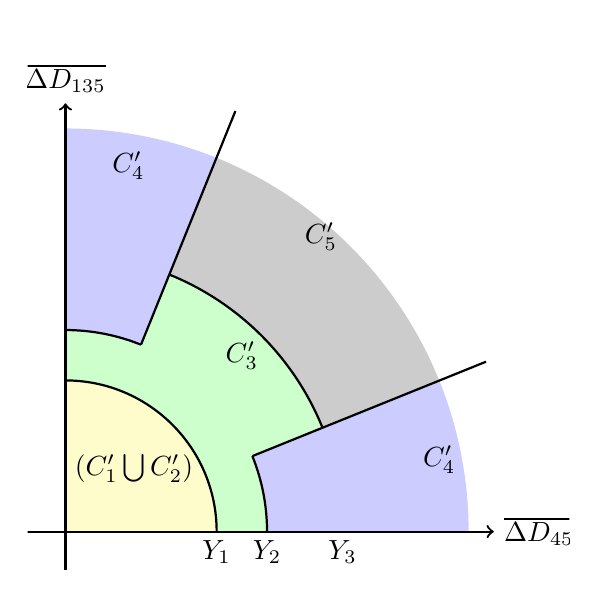
\begin{tikzpicture}[scale=3.2]\clip (-0.15,-0.15) rectangle (2,2);

\fill[fill=black!20] (0,0) -- (22:1.6) arc (22:68:1.6) node[below right=20pt,text width=1cm,text centered] {$C'_5$};

\fill[fill=green!20] (0,0) -- (0:1.1) arc (0:90:1.1);
\draw[thick] (1.1,0) arc (0:90:1.1);

\fill[fill=blue!20] (0,0) -- (68:1.6) arc (68:90:1.6) node[below right=5pt,text width=1cm,text centered] {$C'_4$};
\fill[fill=blue!20] (0,0) -- (0:1.6) arc (0:22:1.6)  node[below=20pt,text width=2cm,text centered] {$C'_4$};
\draw[thick] (0,0) -- (68:1.8);
\draw[thick] (0,0) -- (22:1.8);

\fill[fill=green!20] (0,0) -- (0:0.8) arc (0:90:0.8);
\draw (0.7,0.7) node {$C'_3$};
\draw[thick] (0.8,0) arc (0:22:0.8);
\draw[thick] (0,0.8) arc (90:68:0.8);

\fill[fill=yellow!20] (0,0) -- (0:0.6) arc (0:90:0.6);
\draw (0.35,0.25) node[text width=2cm] {($C'_1\bigcup C'_2$)};
\draw[thick] (0.6,0) arc (0:90:0.6);

\draw[thick, ->] (-1.7,0) -- (1.7,0) node[right] {$\overline{\Delta D_{45}}$};
\draw[thick, ->] (0,-1.7) -- (0,1.7) node[above] {$\overline{\Delta D_{135}}$};

\draw (0.6,-0.08) node{$Y_1$};
\draw (0.8,-0.08) node{$Y_2$};
\draw (1.1,-0.08) node{$Y_3$};
\end{tikzpicture}}\\
	\caption{Espaces permettant la classification des blocs.}
\end{figure}

Comme précédemment, chaque tube est localisé dans un espace $\Psi'=(\overline{\Delta D_{45}}, \overline{\Delta D_{135}})$, formé de manière identique à $\Psi$ et présenté sur la figure~\ref{fig:deltaD}. Dans ce nouveau plan, un tube dont les caractéristiques se situent dans la région étiquetée ($C'_1\bigcup C'_2$) appartient à une zone homogène. Si elles se situent dans $C'_3$ ou $C'_4$, alors il appartient respectivement à une zone de textures fines ou de contours. Si elles sont dans $C'_5$, le tube appartient à une zone de textures fortes.

Enfin, la distinction entre les tubes des classes $C_1$ et $C_2$ correspondant respectivement aux zones uniformes de luminance faible et aux zones uniformes de luminance moyenne et forte se fait à l'aide d'un seuil. Nous considérons qu'une zone est de faible luminance si sa luminance moyenne est inférieure à un cinquième de la dynamique environ. C'est pourquoi, si le tube a un niveau de gris moyen sur l'ensemble de ces pixels inférieur à 50 sur l'échelle $[\text{0};\text{255}]$, il est assigné à la classe $C_1$. Sinon, il appartient à la classe $C_2$. La classification se termine une fois chaque tube de la séquence classé. Les objets en mouvement le long de la séquence entière sont ainsi suivis. Les tubes voisins et appartenant à la même classe se regroupent naturellement en un volume spatio-temporel de cette classe.


\subsubsection{Assurer une cohérence temporelle}
Si la classification d'un tube était uniquement assurée par le calcul des gradients, des discontinuités importantes pourraient apparaitre. Afin d'obtenir une classification cohérente d'un tronçon à l'autre, un suivi des tubes de proche en proche est réalisé. Pour cela, les tubes spatio-temporels qui se suivent temporellement sont assemblés afin de constituer des régions spatio-temporelles sur la séquence entière. Ceci est illustré par la figure~\ref{fig:overlapTubes}. Cet assemblage consiste à regrouper un tube d'un tronçon avec le tronçon suivant pour faire correspondre des tubes qui se suivent temporellement. Cela permet de prolonger les tubes d'un tronçon à l'autre en cumulant les gradients sur une durée supérieure à un tube. La classification se fait alors sur cet ensemble de tubes, assurant une cohérence temporelle.

\begin{figure}[htbp]
	\centering
	\begin{tikzpicture}[scale=1.5]
		% \begin{tikzpicture}[scale=2.5]

% jointure derrière les tubes
\draw(0.9,-0.8)--(3.9,-0.4);
\draw(4.3,-0.3)--(7.6,0.5);
\draw[dashed](4.3,-0.3)--(3.9,-0.4);

% blocs rouges
\filldraw[fill=red!40] (0.7,-0.7) -- (0.9,-0.5) --  (0.9,-0.8) -- (0.7,-1) -- cycle;
\filldraw[fill=red!40] (1.45,-0.6) -- (1.65,-0.4) --  (1.65,-0.7) -- (1.45,-0.9) -- cycle;
\filldraw[fill=red!40] (2.2,-0.5) -- (2.4,-0.3) --  (2.4,-0.6) -- (2.2,-0.8) -- cycle;
\filldraw[fill=red!40] (2.95,-0.4) -- (3.15,-0.2) --  (3.15,-0.5) -- (2.95,-0.7) -- cycle;
\filldraw[fill=red!40] (3.7,-0.3) -- (3.9,-0.1) --  (3.9,-0.4) -- (3.7,-0.6) -- cycle;

% blocs bleus
\filldraw[fill=blue!40] (4.1,-0.2) -- (4.3,0) --  (4.3,-0.3) -- (4.1,-0.5) -- cycle;
\filldraw[fill=blue!40] (4.925,0) -- (5.125,0.2) --  (5.125,-0.1) -- (4.925,-0.3) -- cycle;
\filldraw[fill=blue!40] (5.75,0.2) -- (5.95,0.4) --  (5.95,0.1) -- (5.75,-0.1) -- cycle;
\filldraw[fill=blue!40] (6.575,0.4) -- (6.775,0.6) --  (6.775,0.3) -- (6.575,0.1) -- cycle;
\filldraw[fill=blue!40] (7.4,0.6) -- (7.6,0.8) --  (7.6,0.5) -- (7.4,0.3) -- cycle;

% jointure inter-tube
\draw[dashed](4.1,-0.2)--(3.7,-0.3);
\draw[dashed](4.3,0)--(3.9,-0.1);
\draw[dashed](4.1,-0.5)--(3.7,-0.6);

% images
\foreach \j in {0,1,2,3,4,5,6,7,8,9} % grille sur les autres images
{
	\draw[help lines](0.75*\j,0)--(1 + 0.75*\j,1)--(1+0.75*\j,-1)--(0.75*\j,-2)--cycle;
}

% tubes
\draw(0.7,-0.7)--(3.7,-0.3);
\draw(0.7,-1)--(3.7,-0.6);
\draw(0.9,-0.5)--(3.9,-0.1);
\draw(4.1,-0.2)--(7.4,0.6);
\draw(4.3,0)--(7.6,0.8);
\draw(4.1,-0.5)--(7.4,0.3);

% labels
\path (0,-2.2) node {$i-2$}  -- (0.75,-2.2) node {$i-1$} -- (1.5,-2.2) node {$i$} -- (2.25,-2.2) node {$i+1$} -- (3,-2.2) node {$i+2$} -- (3.75,-2.2) node {$i+3$} -- (4.5,-2.2) node {$i+4$} -- (5.25,-2.2) node {$i+5$} -- (6,-2.2) node {$i+6$} -- (6.75,-2.2) node {$i+7$};
\path (1.5,1.5);


% \end{tikzpicture}
	\end{tikzpicture}
	\caption{Schéma de la fusion des tubes se chevauchant.}
  \label{fig:overlapTubes}
\end{figure}


\subsubsection{Paramétrage de la création du partitionnement des espaces \texorpdfstring{$\Psi$}{Psi} et \texorpdfstring{$\Psi'$}{Psi'}} \label{ssec:paramClass}
Les paramètres permettant de modifier la classification sont les angles et les rayons délimitant les régions des espaces $\Psi$ et $\Psi'$. Le rayon de la région $C_1$ est nommé $Y_1$, le premier de la région $C_3$ est nommé $Y_2$ et le second $Y_3$. L'angle le plus petit est nommé $A_1$, alors que le plus grand est nommé $A_2$. Réduire ou augmenter les valeurs de ces paramètres influent sur les tailles des régions spatio-temporelles et donc sur l'appartenance d'un tube à telle ou telle classe.

Diverses combinaisons de paramètres ont été testées, indépendamment pour chaque contenu. Un ensemble de paramètre pertinent permet de bien distinguer les zones spatio-temporelles principales de la séquence. Une telle vérification peut se faire visuellement. Ainsi, les paramètres ont été déterminées de manière à obtenir une classification aussi réaliste que possible.


\subsection{Conclusion}
Dans cette section, nous avons présenté la méthode de segmentation spatio-temporelle et de classification utile à notre étude. Cette méthode est effectuée en deux phases. La première consiste à segmenter temporellement des séquences en tubes élémentaires. Ceux-ci ont la particularité de suivre le mouvement local et ainsi de conserver un contenu cohérent. La seconde phase classe chaque tube suivant l'activité spatiale de son contenu. La cohérence temporelle est assurée par un suivi de proche en proche des tubes.


\section{Mise en \oe uvre de la méthodologie}
Afin de tester la méthodologie proposée, nous avons utilisé les douze contenus de l'ensemble SVT2006 décrits dans la section~\ref{ssec:seq-svt2006} et les séquences dégradées par le codage \avc{} correspondantes. À partir de ces données, nous avons généré des séquences partiellement dégradées. Le tableau~\ref{tab:paramClasses} donne les valeurs des paramètres de la création des régions pour chaque contenu. Ces paramètres ont été déterminés après visualisation des séquences. Plusieurs étapes sont requises pour générer les séquences finales comme le montre la figure~\ref{fig:miseEnOeuvre}. La première de ces étapes est la génération d'une séquence vidéo contenant en chaque pixel une représentation de la classe du pixel correspondant dans la séquence d'origine. Cette séquence est utilisée pour substituer les pixels dégradés aux pixels originaux. Des traitements sont utilisés pour assurer la segmentation totale de la séquence et pour adoucir la visibilité des transitions.

\begin{figure}[htbp]
	\centering
	\begin{tikzpicture}[scale=1.5, text width=2.5cm, node distance=3.2cm, text centered]
		\node[text width=1.4cm] (seq) {tubes classifiés};
		\node[action, right of=seq, node distance=3cm] (seg) {génération des séquences de classes};
		\node[action, right of=seg] (comp) {complétion de la segmentation};
		\node[action, right of=comp] (gene) {génération des séquences partiellement dégradées};
		\node[right of=gene, text width=2cm] (out) {séquences partiellement dégradées};
		\draw[fleche] (seq) -- (seg);
		\draw[fleche] (seg) -- (comp);
		\draw[fleche] (comp) -- (gene);
		\draw[fleche] (gene) -- (out);
	\end{tikzpicture}
	\caption{Étapes de la génération des séquences partiellement dégradées.}
  \label{fig:miseEnOeuvre}
\end{figure}

\begin{table}[htbp]
\centering
\begin{tabular}{cccccc}\toprule
\strong{contenu}					& $A_1$ & $A_2$ & $Y_1$ & $Y_2$ & $Y_3$ \\ \toprule
\emph{Above Marathon}			& 20 & 70 & 8 & 10 & 13\\ \midrule
\emph{Captain}						& 20 & 70 & 8 & 10 & 13\\ \midrule
\emph{Dance in the Woods}	& 20 & 70 & 8 & 10 & 13\\ \midrule
\emph{Duck Fly}						& 10 & 80 & 8 & 10 & 13\\ \midrule
\emph{Fountain Man}				& 25 & 65 & 8 & 10 & 13\\ \midrule
\emph{Group Disorder}			& 20 & 70 & 10 & 15 & 20\\ \midrule
\emph{Inside Marathon}			& 20 & 70 & 10 & 15 & 20\\ \midrule
\emph{New Parkrun}				& 20 & 70 & 8 & 10 & 13\\ \midrule
\emph{Rendezvous}				& 20 & 70 & 8 & 10 & 13\\ \midrule
\emph{Stockholm Travel}		& 25 & 65 & 8 & 10 & 13\\ \midrule
\emph{Tree Pan}						& 20 & 70 & 8 & 10 & 13\\ \midrule
\emph{Ulriksdals}					& 20 & 70 & 8 & 10 & 13\\ \bottomrule
\end{tabular}
\caption{Valeurs des paramètres de création des régions pour chaque contenu.}
\label{tab:paramClasses}
\end{table}


\subsection{Résultats de la classification}
Le procédé de classification fournit les classes de chaque tube. Chaque classe représente une certaine proportion du contenu total. Ces proportions sont présentées dans le tableau~\ref{tab:proportionsClasses}. Nous remarquons que la classe $C_1$ couvre une gamme de proportions allant de pratiquement zéro (0,13\%) à 42\%. La classe $C_2$ couvre la plus large gamme de valeurs. Les vidéos contenant de l'eau qui tombent comme \emph{Captain} ou \emph{Fountain Man} ont une proportion particulièrement élevée de zones de type $C_2$ avec plus de 78\%. Ceci est dû à la classification dans $C_2$ des zones de chute d'eau. Les classes $C_3$ et $C_4$ ont une forte importance, entre 6\% et 54\% pour la première et entre 0.36\% à plus de 60\% pour la dernière. Enfin, la classe $C_5$ a une importance particulièrement faible, en dessous de 3\% sauf pour deux vidéos. Ces proportions sont consistantes avec la nature du contenu. Ceux-ci sont réalistes avec des scènes en extérieur. Ainsi, nous y trouvons peu de contours, quelques zones homogènes comme le ciel ou les vêtements et beaucoup de textures comme les arbres et l'herbe.

\begin{table}[htbp]
\centering
\begin{tabular}{cccccc} \toprule
\strong{contenu}					& $C_1$ & $C_2$ & $C_3$ & $C_4$ & $C_5$ \\ \toprule
\emph{Above Marathon}			& 3,75 & 17,45 & 27,79 & 50,06 & 0,94\\\midrule
\emph{Captain}						& 13,14 & 78,26 & 6,81 & 0,36 & 1,43 \\\midrule
\emph{Dance in the Woods}	& 3,80 & 22,57 & 53,86 & 16,75 & 3,02 \\\midrule
\emph{Duck Fly}						& 0,13 & 8,97 & 19,50 & 60,70 & 10,70\\\midrule
\emph{Fountain Man}				& 10,52 & 70,71 & 13,37 & 3,94 & 1,46 \\\midrule
\emph{Group Disorder}			& 25,28 & 38,59 & 29,80 & 4,54 & 1,79\\\midrule
\emph{Inside Marathon}			& 5,64 & 47,64 & 39,77 & 6,75 & 0,20 \\\midrule
\emph{New Parkrun}				& 41,89 & 32,98 & 17,67 & 3,49 & 3,97 \\\midrule
\emph{Rendezvous}				& 8,78 & 12,38 & 19,87 & 56,91 & 2,05 \\\midrule
\emph{Stockholm Travel}		& 8,02 & 58,63 & 14,23 & 1,53 & 17,59\\\midrule
\emph{Tree Pan}						& 1,96 & 16,63 & 22,58 & 58,15 & 0,68 \\\midrule
\emph{Ulriksdals}					& 13,54 & 41,31& 40,48 & 3,31 & 1,36 \\\bottomrule
\end{tabular}
\caption{Proportions des classes de chaque contenu exprimées en pourcentage.}
\label{tab:proportionsClasses}
\end{table}


\subsection{Création de masques de classes}
À partir des classes des tubes d'une séquence, une séquence de classes est générée. Il s'agit d'assigner une valeur particulière de luminance à chaque pixel appartenant à une classe donnée. Ceci permet de repérer visuellement les zones spatio-temporelles. La figure~\ref{fig:videoClasse} présente un exemple de classification obtenue par notre méthode. Bien sûr, elle ne rend pas compte de l'aspect temporel de celle-ci.

\begin{figure}[htbp]
	\centering
	\includegraphics[width=0.98\linewidth]{img/chap3/videoClasseMobcalOrdered}
	\begin{tikzpicture}
		\draw[legende] (-2.5,-4.4) rectangle (2.5,-5);
		\node at (0,-4.7) {\includegraphics[scale=7]{img/chap3/legendClasse1} $C_1$ \includegraphics[scale=7]{img/chap3/legendClasse2} $C_2$ \includegraphics[scale=7]{img/chap3/legendClasse3} $C_3$ \includegraphics[scale=7]{img/chap3/legendClasse4} $C_4$ \includegraphics[scale=7]{img/chap3/legendClasse5} $C_5$};
	\end{tikzpicture}
	\caption{Image de la séquence des classes du contenu New Mobile \& Calendar.}
	\label{fig:videoClasse}
\end{figure}

Tous les pixels de l'image centrale d'un tronçon sont assignés à une classe. Cependant, la méthode de création des tubes laisse des pixels sans classification sur les autres images. Parallèlement, elle provoque aussi le recouvrement partiel de tubes à d'autres endroits. La segmentation n'est donc pas complète. Afin de créer des séquences dont tous les pixels sont étiquetés, nous leur assignons tous une classe en affectant à un pixel non étiqueté la classe du tube le plus proche spatialement. La même méthode est utilisée pour déterminer la classe d'un pixel où se recouvre plusieurs tubes. La figure~\ref{fig:avecTrous} présente un exemple de vidéos de classe avant ce traitement. La figure~\ref{fig:sansTrous} présente ce même exemple après ce traitement. Ainsi, chaque pixel du contenu traité appartient à une unique classe.

\begin{figure}[htbp]
	\centering
	\subfloat[\label{fig:avecTrous}Avant traitement.]{\includegraphics{img/chap3/avantRemplissageTrousOrdered}}\hfill
	\subfloat[\label{fig:sansTrous}Après traitement.]{\includegraphics{img/chap3/apresRemplissageTrousOrdered}}\\
	\begin{tikzpicture}
		\draw[legende] (-3.5,-4.4) rectangle (3.5,-5);
		\node at (0,-4.7) {\includegraphics[scale=7]{img/chap3/legendTrou} sans étiquette \includegraphics[scale=7]{img/chap3/legendClasse1} $C_1$ \includegraphics[scale=7]{img/chap3/legendClasse2} $C_2$ \includegraphics[scale=7]{img/chap3/legendClasse3} $C_3$ \includegraphics[scale=7]{img/chap3/legendClasse4} $C_4$ \includegraphics[scale=7]{img/chap3/legendClasse5} $C_5$};
	\end{tikzpicture}
	\caption{Comparaison de deux vidéos de classe, la première avant suppression des zones sans classes et des ambiguïtés de classification, la seconde après.}
\end{figure}


\subsection{Génération des séquences partiellement dégradées}
Les séquences partiellement dégradées sont générées à partir du contenu original, de sa segmentation et classification et des séquences codées à différents débits par \avc{} correspondantes. Les segments d'une séquence dégradée correspondant à une classe sont insérées dans le contenu original. Ce procédé crée une séquence dégradée par classe et par débit. Seuls les segments de la séquence d'une classe donnée sont ainsi dégradés, les autres segments étant ceux de la vidéo d'origine. Les étapes sont présentées sur la figure~\ref{fig:etapesSeqPartDeg} avec seulement le quart de la première image du contenu \emph{Above Marathon}. L'image~\ref{fig:aM-2M-C1} représente les différents segments avec leur classe. L'image~\ref{fig:aM-MC} montre l'image dégradée partiellement : seuls les segments de classe $C_1$ sont dégradés. Ceci est visible sur l'arbre central. Nous créons ainsi cinq séquences partiellement dégradées par contenu et par débit. Pour cette étude, vingt débits ont été sélectionnés par des experts. Ils sont donnés dans le tableau~\ref{tab:debitsClasses}. Par ailleurs, les bordures entre une zone dégradée et une zone d'origine pouvant être visibles, nous les avons adoucies à l'aide d'une fonction d'apodisation d'extension spatiale d'une dizaine de pixels.

\begin{figure}[htbp]
	\centering
	\subfloat[\label{fig:aM}Image du contenu original.]{\includegraphics[scale=0.56]{img/chap3/aboveMarathon}}\\
	\subfloat[\label{fig:aM-2M-C1}Image de la vidéo de classes.]{\includegraphics[scale=0.56]{img/chap3/aboveMarathonMetaClassesOrdered}}\\
	\begin{tikzpicture}
		\draw[legende] (-2.5,0.3) rectangle (2.5,-0.3);
		\node {\includegraphics[scale=7]{img/chap3/legendClasse1} $C_1$ \includegraphics[scale=7]{img/chap3/legendClasse2} $C_2$ \includegraphics[scale=7]{img/chap3/legendClasse3} $C_3$ \includegraphics[scale=7]{img/chap3/legendClasse4} $C_4$ \includegraphics[scale=7]{img/chap3/legendClasse5} $C_5$};
	\end{tikzpicture}\\
	\subfloat[\label{fig:aM-MC}Image de la séquence partiellement dégradée. Les segments de la classe $C_1$ sont ici seuls dégradés.]{\includegraphics[scale=0.56]{img/chap3/aboveMarathon-2M-class1}}\\
	\caption{Les trois étapes de création des séquences partiellement dégradées.}
	\label{fig:etapesSeqPartDeg}
\end{figure}


\begin{table}[htbp]
\centering
\begin{tabular}{cc}\toprule
\textbf{contenu}						& \textbf{débits (Mbps)} \\ \toprule
\emph{Above Marathon}			& 5 ; 8 ; 10	\\\midrule
\emph{Captain	}						& 1 ; 3 ; 5		\\\midrule
\emph{Dance in the Woods}	& 3 ; 5 ; 6		\\\midrule
\emph{Duck Fly}						& 4 ; 6 ; 8		\\\midrule
\emph{Fountain Man}				& 1 ; 5			\\\midrule
\emph{Group Disorder}			& 2 ; 4			\\\midrule
\emph{Rendezvous}				& 6 ; 8			\\\midrule
\emph{Ulriksdals}					& 1 ; 4			\\\bottomrule
\end{tabular}
\caption{Débits en Mbps utilisés pour la création de séquences partiellement dégradées.}
\label{tab:debitsClasses}
\end{table}


\subsection{Évaluation subjective de la qualité des séquences dégradées}
Afin de disposer des notes de qualité de chacune des séquences partiellement dégradées, nous effectuons une campagne de tests. La mesure obtenue est liée à l'impact d'une classe donnée sur la qualité perçue pour le niveau de dégradation créé par le codage au débit considéré. Les tests ont été réalisés dans les mêmes conditions que pour l'évaluation de la qualité visuelle des vidéos de la base de l'annexe~\ref{annex:base}. Une session SAMVIQ pour un contenu donné et à un débit $B$ est composée :

\begin{enumerate}
\item du contenu de référence explicite, servant d'ancre de haute qualité ;
\item de la séquence partiellement dégradée par la classe $C_1$, codé au débit $B$ ;
\item de la séquence partiellement dégradée par la classe $C_2$, codé au débit $B$ ;
\item de la séquence partiellement dégradée par la classe $C_3$, codé au débit $B$ ;
\item de la séquence partiellement dégradée par la classe $C_4$, codé au débit $B$ ;
\item de la séquence partiellement dégradée par la classe $C_5$, codé au débit $B$ ;
\item de la séquence entièrement dégradée, par le codage au débit $B$ ;
\item d'une séquence entièrement dégradée à bas débit, servant d'ancre de basse qualité ;
\item d'une séquence entièrement dégradée à un débit moyen, choisi selon $B$ et le bas débit ;
\item de la référence cachée.
\end{enumerate}

Une session permet donc de recueillir à la fois les notes de qualités de chaque séquence entièrement dégradée et celles de toutes les séquences partiellement dégradées.


\subsection{Conclusion}
Nous avons présenté la méthode de segmentation spatio-temporelle et de classification de séquences vidéo que nous avons conçue afin de mesurer l'impact des dégradations dans chaque type de segment spatio-temporel. Cela nous a permis de connaitre les pertes de qualité liées à chaque classe séparément. Nous avons également mesuré les pertes de qualité quand l'ensemble de la séquence est dégradé. Celles-ci sont issues des tests de qualité de la base de l'annexe~\ref{annex:base}. Il ne reste désormais plus qu'à tenter de relier les impacts visuels des dégradations locales à celle des dégradations globales.


\section{De la perte de qualité subjective locale à l'estimation globale} \label{sec:deLocalAGlobal}
Nous cherchons à savoir s'il est possible de relier les pertes de qualité locales d'un côté et la perte de qualité globale de l'autre. Il n'est pas évident a priori qu'une telle relation soit simple, étant donné que le cumul correspondant est fait au niveau du cerveau humain au cours de l'évaluation subjective de qualité. Si nous pouvons identifier cette relation, cela sera très intéressant pour construire un modèle objectif de qualité. En effet, celui-ci pourrait alors évaluer séparément chaque classe de contenu avant de cumuler les qualités locales en une note de qualité globale.

Commençons par clarifier les termes utilisés. La note de qualité visuelle du contenu $S_j$ non dégradé est notée MOS$(S_j)$. Dans la méthodologie SAMVIQ, elle correspond à la note de la référence cachée. La note de la séquence entièrement dégradée à un débit $B_k$ correspondante est notée MOS$(S_j,B_k)$. De plus, une note de qualité partielle, notée MOS($S_j, B_k, C_i$), est obtenue pour chaque contenu $S_j$, codé au débit $B_k$ et avec une dégradation présente uniquement sur les segments de classe $C_i$. La différence entre MOS$(S_j)$ et MOS$(S_j,B_k)$ représente la perte de qualité globale de la séquence. Nous la notons DMOS$(S_j,B_k)$. La différence entre une note de qualité partielle MOS($S_j, B_k, C_i$) et la note de qualité MOS$(S_j)$ est appelée $\Delta$MOS($C_i, S_j, B_k$). Elle indique la perte de qualité induite par les dégradations de la classe $C_i$. Pour un contenu $S_j$ et un débit $B_k$ donnés, la relation recherchée est donc entre DMOS$(S_j,B_k)$ et les cinq valeurs $\Delta$MOS($C_i, S_j, B_k$) avec $i\in [\text{1};\text{5}]$. La figure~\ref{fig:DMOSDeltaMOS} représente les différentes valeurs présentes dans ce type de relation. Sur une échelle de qualité allant de 0 à 100, la valeur MOS$(S_j)$ est la note maximale obtenue et MOS$(S_j,B_k)$ la note minimale. Les $\Delta$MOS($C_i, S_j, B_k$) sont donc compris entre ces deux extrêmes.

Plusieurs modèles de cumul ont été testés dans le but d'établir la relation cherchée. Nous présentons ici les plus intéressants. Nous distinguerons deux catégories : les modèles linéaires et les non linéaires.

\begin{figure}[htbp]
	\centering
	\begin{tikzpicture}[yscale=1.5]% échelle
\draw[->,-latex,very thick] node[left=72pt] {0} (-3,0) -- node[anchor=west,pos=1] {100} (-3,10);

% ref et deg
\draw[thick,dashed] (-3,9) -- (2.5,9) node[right]{MOS$(S_j)$};
\draw[thick,dashed] (-3,2) -- (2.5,2) node[right]{MOS$(S_j,B_k)$};

% DMOS
\draw[<->,latex-latex,thick] (-4,2) -- node[left]{DMOS$(S_j,B_k)$} (-4,9);

% DeltaMOS des classes
\draw[<->,latex-latex,thick] (-2,5) 	-- node[above,pos=0,rotate=90]	{$\Delta$MOS$(S_j,C_1,B_k)$} (-2,9);
\draw[<->,latex-latex,thick] (-1,4) 	-- node[above,pos=0,rotate=90]	{$\Delta$MOS$(S_j,C_2,B_k)$} (-1,9);
\draw[<->,latex-latex,thick] (0,6) 	-- node[above,pos=0,rotate=90]	{$\Delta$MOS$(S_j,C_3,B_k)$} (0,9);
\draw[<->,latex-latex,thick] (1,7) 	-- node[above,pos=0,rotate=90]	{$\Delta$MOS$(S_j,C_4,B_k)$} (1,9);
\draw[<->,latex-latex,thick] (2,3) 	-- node[above,pos=0,rotate=90]	{$\Delta$MOS$(S_j,C_5,B_k)$} (2,9);

\end{tikzpicture}
	\caption{Représentation des différentes valeurs présentes dans la relation entre la perte de qualité globale, notée DMOS$(S_j,B_k)$, et les pertes locales notées $\Delta$MOS($C_i, S_j, B_k$) avec $i\in [\text{1};\text{5}]$.}
	\label{fig:DMOSDeltaMOS}
\end{figure}


\subsection{Modèles linéaires} \label{ssec:modeleLin}
Ces modèles, les plus simples consistent à calculer le DMOS du contenu $S_j$ au débit $B_k$ par :
\begin{equation}
\text{DMOS}(S_j,B_k) = \sum_{\substack{1\le i \le 5}}\Delta\text{MOS}(C_i, S_j, B_k) \times \delta_i
\end{equation}
%
avec $\delta_i$ valant 0 ou 1. Ainsi, soit la contribution d'une classe est prise en compte entièrement, soit elle ne l'est pas du tout. En effet, ceci nous renseignera sur l'importance relative de chaque classe sur le cumul. Il y a ainsi 31 modèles différents possibles. Nous évaluons les performances de chacun d'eux par deux critères : le coefficient de corrélation linéaire et l'écart-type de la différence, noté $\sigma_e$. Cet écart-type est calculé entre les $\Delta$MOS$_i$ et leurs prédictions linéaires $\Delta$MOSp$_i$ issues d'un modèle donné $X$. La prédiction consiste à calculer  :
\begin{equation}
\Delta\text{MOSp}_i = \left(\rho_{X\Delta} \times \left(\frac{X_i - \overline{X}}{\sigma_X}\right) \times \sigma_\Delta \right) + \overline{\Delta}
\end{equation}
%
avec $\rho_{X\Delta}$ le coefficient de corrélation entre les notes $X_i$ issues du modèle $X$ et les $\Delta$MOS$_i$, $\overline{X}$ la moyenne des $X_i$, $\sigma_X$ l'écart-type des $X_i$, $\overline{\Delta}$ la moyenne des $\Delta$MOS$_i$ et $\sigma_\Delta$ l'écart-type des $\Delta$MOS$_i$.

Le tableau~\ref{tab:combination} présente certains des modèles proposés avec le coefficient de corrélation et la racine carrée de l'erreur quadratique moyenne qu'ils donnent. Pour les modèles dont le coefficient de corrélation est inférieur à 0,9, seuls ceux issus de l'utilisation d'une seule classe sont présentés. Le nom de chaque modèle est symbolisé par la somme des classes prises en compte dans celui-ci.

\begin{table}[htbp]
\centering
\begin{tabular}{ccc}\toprule
\textbf{modèle}					& \textbf{coefficient de corrélation}		& $\sigma_e$ \\ \toprule
$C_2+C_4+C_5$					& 0,9485			& 4,11			\\\midrule
$C_2+C_4$							& 0,9440			& 4,28			\\\midrule
$C_2+C_3+C_5$					& 0,9094			& 5,40			\\\midrule
$C_1+C_2+C_3+C_4+C_5$	& 0,9058			& 5,50			\\\midrule
$C_1+C_2+C_4+C_5$			& 0,9052			& 5,52			\\\midrule
$C_2+C_3+C_4+C_5$			& 0,9041			& 5,55			\\\midrule
$\cdots$								& $\cdots$		& $\cdots$	\\\midrule
% $C_2+C_3$						& 0,8978			& \\\midrule
% $C_1+C_2+C_4$				& 0,8939			& \\\midrule
% $C_1+C_2+C_3+C_4$		& 0,8936			& \\\midrule
% $C_2+C_3+C_4$				& 0,8892			& \\\midrule
% $C_1+C_4+C_5$				& 0,8739			& \\\midrule
% $C_1+C_2+C_3+C_5$		& 0,8447			& \\\midrule
% $C_1+C_3+C_4+C_5$		& 0,8442			& \\\midrule
% $C_1+C_4$						& 0,8379			& \\\midrule
% $C_1+C_2+C_3$				& 0,8291			& \\\midrule
% $C_1+C_3+C_4$				& 0,8183			& \\\midrule
% $C_1+C_3+C_5$				& 0,7995			& \\\midrule
% $C_2+C_5$						& 0,7765			& \\\midrule
$C_2$									& 0,7664			& 8,33			\\\midrule
% $C_1+C_3$						& 0,7635			& \\\midrule
% $C_3+C_4+C_5$				& 0,7515			& \\\midrule
% $C_3+C_5$						& 0,7154			& \\\midrule
% $C_4+C_4$						& 0,7154			& \\\midrule
% $C_3+C_4$						& 0,7130			& \\\midrule
$C_3$									& 0,7094			& 9,15			\\\midrule
% $C_1+C_2+C_5$				& 0,7073			& \\\midrule
% $C_1+C_2$						& 0,6810			& \\\midrule
$C_4$									& 0,6400			& 9,97			\\\midrule
% $C_1+C_5$						& 0,6102			& \\\midrule
$C_5$									& 0,5472			& 10,86		\\\midrule
$C_1$									& 0,5349			& 10,96		\\\bottomrule
\end{tabular}
\caption{Modèles linéaires de cumul des pertes de qualité locales accompagnés de leur performances respectives.}
\label{tab:combination}
\end{table}

Les performances révèlent l'importance relative de chaque classe dans le processus de cumul effectué par l'observateur moyen. Malgré sa simplicité, une telle approche permet de bonnes corrélations avec quelques classes stratégiques. La combinaison des seules zones homogènes de forte luminance $C_2$ et des zones de textures fortes $C_4$ fournit une très bonne corrélation avec le jugement humain. Ceci s'explique notamment par la nature des contenus, composés en majorité de ce type de zones. Malgré ses faibles proportions et ses mauvaises performances individuelles, la classe des contours $C_5$ est présente dans cinq des six premiers modèles les plus performants. Ainsi, l'ensemble des dégradations de ces trois classes $C_2$, $C_4$ et $C_5$ sont étroitement liées à la qualité globale de la séquence. Leur impact sur la perception de la qualité par l'observateur moyen est donc particulièrement important.

À l'opposé, lorsqu'une seule classe est utilisée, nous obtenons parmi les plus mauvaises performances. Cela signifie que la qualité d'une seule classe de contenu ne suffit pas à représenter la qualité globale de la séquence, ce qui semble évident a priori. En contrepartie, la combinaison des cinq classes n'obtient pas la meilleure performance, indiquant que certaines zones ne sont pas ou peu prises en compte dans la construction du jugement de qualité de l'observateur moyen. Cela pourrait être affiné avec des valeurs non entières de $\delta$.

Un modèle linéaire simple peut donc suffire à fournir une très bonne corrélation entre la qualité globale et les qualités locales. Ce résultat est très intéressant car il montre que les qualités locales peuvent être cumulées afin d'approcher la qualité globale. Ainsi, nous pouvons passer de l'évaluation de la séquence entière à une évaluation par parties, chacune exploitant la classe de contenu où elle est calculée.


\subsection{Modèles non linéaires}
Des modèles non linéaires peuvent également être envisagés. Le premier que nous proposons est également très simple et ne considère que les valeurs maximales des $\Delta$MOS. Le second est plus évolué et introduit la notion d'unités de dégradation.


\subsubsection{Modèle basé sur les valeurs maximales des pertes locales}
Ce modèle considère que les classes avec la plus grande perte locale contribuent le plus à la perte globale. Il s'exprime par :
\begin{equation}
\text{DMOS}(S_j,B_k) = \max_i \left(\Delta\text{MOS}(C_i, S_j, B_k)\right)
\end{equation}
%
Ainsi, en ne retenant que la classe de plus grand $\Delta$MOS pour chaque contenu, le coefficient de corrélation linéaire vaut 0,9467 et la racine carrée de l'erreur quadratique moyenne vaut 4,179. Si la somme des deux classes qui contribuent le plus est utilisée, c'est-à-dire :
\begin{equation}
\text{DMOS}(S_j,B_k) = \max_i \left(\Delta\text{MOS}(C_i, S_j, B_k)\right) + \max_{l, l\neq i} \left(\Delta\text{MOS}(C_l, S_j, B_k)\right)
\end{equation}
%
alors le coefficient de corrélation linéaire vaut 0,9530 et la racine carrée de l'erreur quadratique moyenne vaut 3,933. Les classes retenues sont majoritairement les classes $C_2$ et $C_3$, ce qui confirme leur importance.

Le modèle utilisant les deux classes de plus forte contribution obtient de meilleures performances que tous les modèles linéaires présentés précédemment. L'idée de résumer la perte à ses plus grands contributeurs est donc bonne. Cependant, l'inconvénient majeur de cette méthode est qu'elle nécessite la connaissance a priori de toutes les notes de qualités locales afin de pouvoir en sélectionner les valeurs maximales.


\subsubsection{Modèle de prédiction des qualités basé sur l'unité de dégradation}
Ce modèle ne prédit pas les pertes de qualité locales, mais directement les notes de qualité, c'est-à-dire les MOS. Il exploite pour cela la notion d'unité de dégradation~\cite{ccir}. La définition de l'unité de dégradation $U_{\mathit{ijk}}$ associée à la qualité $Q_{\mathit{ijk}} =$ MOS($C_i, S_j, B_k$) de la classe $C_i$ du contenu $S_j$ au débit $B_k$ est :
\begin{equation}
U_{\mathit{ijk}} = \frac{\hat{Q}_{j} - Q_{\mathit{ijk}}}{Q_{\mathit{ijk}}} = \frac{\hat{Q}_{j}}{Q_{\mathit{ijk}}} - 1
\end{equation}
avec $\hat{Q}_{j} = 100$ la qualité de référence. En effet, nous considérons ici que la qualité de référence doit être optimale, c'est-à-dire que la prise de vue est parfaite. Or dans nos tests, le MOS $Q_{j}$ de la référence cachée est la plus haute valeur et ne vaut jamais 100. C'est pourquoi dans ce modèle, nous appliquons une pondération $w_j$ à chaque MOS du contenu $S_j$ afin de transformer la valeur de la référence cachée pour qu'elle vaille 100 :
\begin{equation}
Q_{\mathit{ijk}}' = w_j \times Q_{\mathit{ijk}} = \frac{100}{Q_{j}}\times Q_{\mathit{ijk}}.
\end{equation}
Un modèle de cumul des unités de dégradation de chaque classe $C_i$ est définie par :
\begin{equation}
U_{jk} = \sum_{i=1}^5 U_{\mathit{ijk}} = \frac{\hat{Q}_{j}}{Q_{\mathit{jk}}} - 1
\end{equation}
et la prédiction de la note de qualité globale du contenu $S_j$ au débit $B_k$ est donc :
\begin{equation}
Q_{\mathit{jk}} = \frac{\hat{Q}_{j}}{1+U_{\mathit{jk}}}.
\end{equation}

Nous utilisons ce modèle pour prédire les MOS des 20 séquences du tableau~\ref{tab:debitsClasses}. Le coefficient de corrélation linéaire entre les MOS subjectifs et les MOS prédits vaut 0,9160. La racine carrée de l'erreur quadratique moyenne vaut 5,934. En considérant uniquement les trois classes les plus significatives, à savoir $C_2$, $C_4$ et $C_5$, le coefficient de corrélation augmente à 0,9583 et l'erreur chute à 4,226. Encore une fois, ne considérer que les classes les plus importantes améliore significativement les performances. Ce modèle obtient ainsi la meilleure corrélation pour une erreur légèrement supérieure à celle des meilleurs modèles linéaires et des modèles basé sur les valeurs maximales des pertes locales.


\subsection{Conclusion}
Nous venons de présenter plusieurs modèles de cumul des pertes de qualités locales en une évaluation de la perte globale de qualité. Seul le dernier est une prédiction directe des notes de qualité. Les meilleurs modèles obtiennent une très bonne corrélation entre les données subjectives et leur prédiction. Le tableau~\ref{tab:MeilleuresCombinaisons} récapitule les meilleures performances de chaque modèle. Le principal enseignement de cette étude est qu'il est possible de trouver une relation entre des évaluations de qualité partielles et l'évaluation de la séquence complète. De plus, les modèles proposés sont tous simples d'utilisation, ce qui renforce leur intérêt.

\begin{table}[htbp]
\centering
\begin{tabular}{ccc}\toprule
\textbf{modèle}							& \textbf{coefficient de corrélation}	& \textbf{reqm}	\\ \toprule
linéaire											& 0,9485												& 4,11\\ \midrule
non linéaire									& 0,9530												& 3,933\\ \midrule
prédiction des notes de qualité 	& 0,9583 												& 4,226\\ \bottomrule
\end{tabular}
\caption{Meilleures performances des modèles de cumul des pertes de qualité locales.}
\label{tab:MeilleuresCombinaisons}
\end{table}


\section{Conclusion}
Ce chapitre a permis de présenter et d'exploiter une méthodologie originale. Son but est de permettre la caractérisation de l'impact d'un système dégradant de type codage sur la qualité visuelle. Dans le cadre de la télévision haute définition, le système de codage retenu suit la norme \avc. Notre approche prolonge les travaux de Farias~\cite{farias-phd} mais nous remplaçons son partitionnement en type de dégradations par un partitionnement en zones spatio-temporelles cohérentes. L'idée étant posée, il fallait ensuite construire une méthode permettant de l'exploiter. Nous avons donc proposé une segmentation spatio-temporelle qui introduit notamment la notion de tubes 3D dont l'originalité est de suivre le mouvement local. Cette segmentation permet de dégrader un contenu par zones spatio-temporelles suivant leur activité spatiale. Chaque zone est ensuite évaluée individuellement, ce qui permet de recueillir les qualités locales de chaque séquence. Ainsi, l'analyse de l'impact du codage sur la qualité visuelle est plus fine. Néanmoins, la méthode est indépendante du système dégradant, elle pourrait être utilisée dans d'autres contextes.

La question à laquelle nous avons ensuite répondu est celle du cumul de ces notes de qualité par type de contenu en une note de qualité globale. Nous avons montré que de simples combinaisons linéaires entre les pertes de qualité par type de contenu et la perte globale de qualité permettaient d'obtenir une relation forte. Ainsi, l'impact sur la qualité globale peut être déduite des impacts sur chaque type de contenu local.


%Ce résultat est très intéressant car il ouvre la voie à un modèle objectif évaluant la quantité de dégradation globale à partir des dégradations locales. %Dans un second temps, nous avons proposé une fonction de gêne pour l'une des zones spatio-temporelles définies. Pour cela, nous avons contruit plusieurs paramètres de contrôle de la quantité de dégradations d'une même zone spatio-temporelle, répondant ainsi à la problématique de l'injection de dégradation dans une classe.


\ornementChapitre
